\documentclass{article}

\usepackage[utf8]{inputenc}
\usepackage{amsmath, enumitem, url}
\usepackage{xcolor}
\usepackage[margin=1in]{geometry}

% For figures.
% Package float, adds the H option which forces figure placement.
% \usepackage[demo]{graphicx}
\usepackage{graphicx, float, subfig}
\graphicspath{ {./figures/} }

\newcommand\todo{\textcolor{red}{\textbf{[TODO:] }}}

\title{Learning end-to-end control for duckiebot driving}
\author{Group: Dropouts}
\date{June 2021}

\begin{document}
\maketitle

\section{Group Information}

Members:
\begin{itemize}
    \item Keyan Pishdadian (keyanp@cs.washington.edu)
    \item Jakub Filipek (balbok@cs.washington.edu)
    \item Kyle Deeds (kdeeds@cs.washington.edu)
\end{itemize}

\noindent Source code for behavior cloning approach:
\newline
\url{https://github.com/keyan/duckiebot_behavior_cloning}

\noindent Source code for reinforcement learning approach:
\newline
\url{https://github.com/balbok0/cse571-sp21-project-2-dropouts}

\section{Task Overview}

In this project we sought to explore methods for learning an end-to-end control policy that would allow the duckiebot to navigate tracks autonomously. Our goal was to enable the duckiebot and have it make a full loop around a track without any major driving infractions, using only monocular camera data. Ideally this system would be robust enough to generalize to new tracks and work on the real robot as well as in simulation.

Inspired by previous efforts in learning end-to-end control for driving using deep reinforcement learning \cite{DBLP:journals/corr/abs-1807-00412} our original plan was to evaluate a selection of reinforcement learning algorithms to solve this task. Knowing that reproducing reinforcement results is difficult and often unsuccessful \cite{henderson2019deep}, we planned to also experiment with a behavior cloning approach inspired by prior work from NVIDIA where a convolutional neural network was trained to steer a car using only image data \cite{DBLP:journals/corr/BojarskiTDFFGJM16}.

\section{Environment Setup}

We performed experimentation and evaluation of our agents in simulation and on the real robot primarily relying on the ``AI Driving Olympics" infrastructure \cite{zilly2019ai}. Our agent was structured into the AIDO submission format and then executed either in simulation or on the real duckiebot. We used the default episode length configuration, which runs agents for 60 seconds.

\subsection{Simulation}

We used the \texttt{gym-duckietown} simulator \cite{gym_duckietown} for training and evaluation of agents when using a reinforcement learning approach, as well as for evaluation when using behavior cloning (through the AIDO submission infrastructure). For reinforcement learning we only ran evaluation on the most simple map type, ``loop\_empty", which is an square map with no obstacles. Evaluations for behavior cloning used a specific ``challenge", \texttt{aido-LF-sim-validation} which runs the agent on a static selection of maps and ranks submissions against other users.

\subsection{Real World}

Evaluation on the real duckiebot was done on four different maps (\ref{fig:maps}), with a 60 second maximum episode duration. Only map2 was used for real robot data collection.

\begin{figure}[H]
\centering
    \subfloat[\centering map1]{{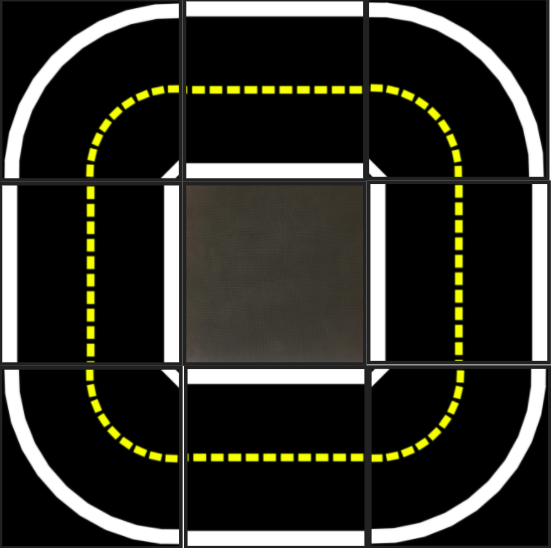
\includegraphics[width=5cm]{map1} }}
    \qquad
    \subfloat[\centering map2]{{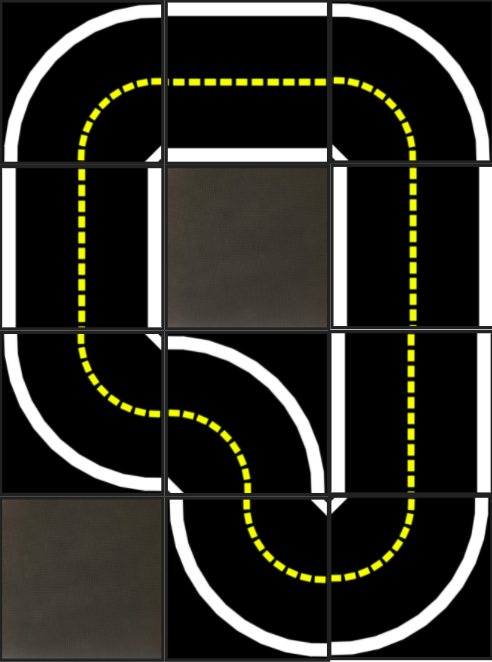
\includegraphics[width=5cm]{map2} }}
    \qquad
    \subfloat[\centering map3]{{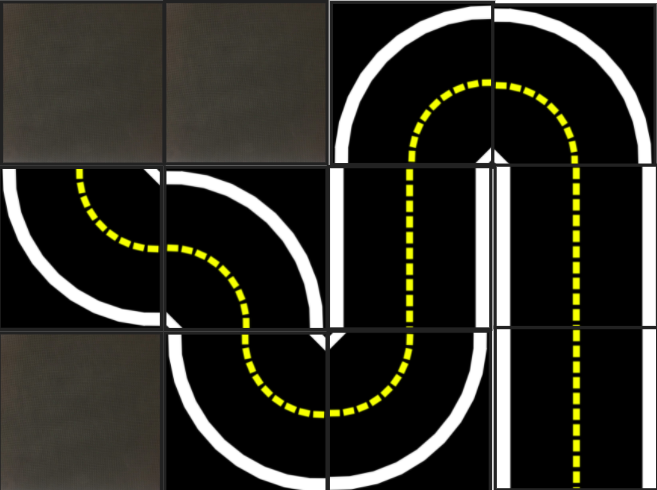
\includegraphics[width=5cm]{map3} }}
    \qquad
    \subfloat[\centering map4]{{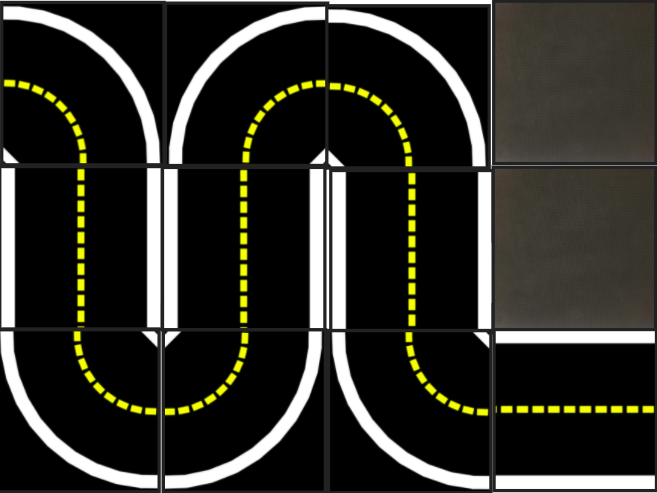
\includegraphics[width=5cm]{map4} }}
    \caption{Digital overview of the four maps used for real-world evaluation.}
    \label{fig:maps}
\end{figure}

\begin{figure}[H]
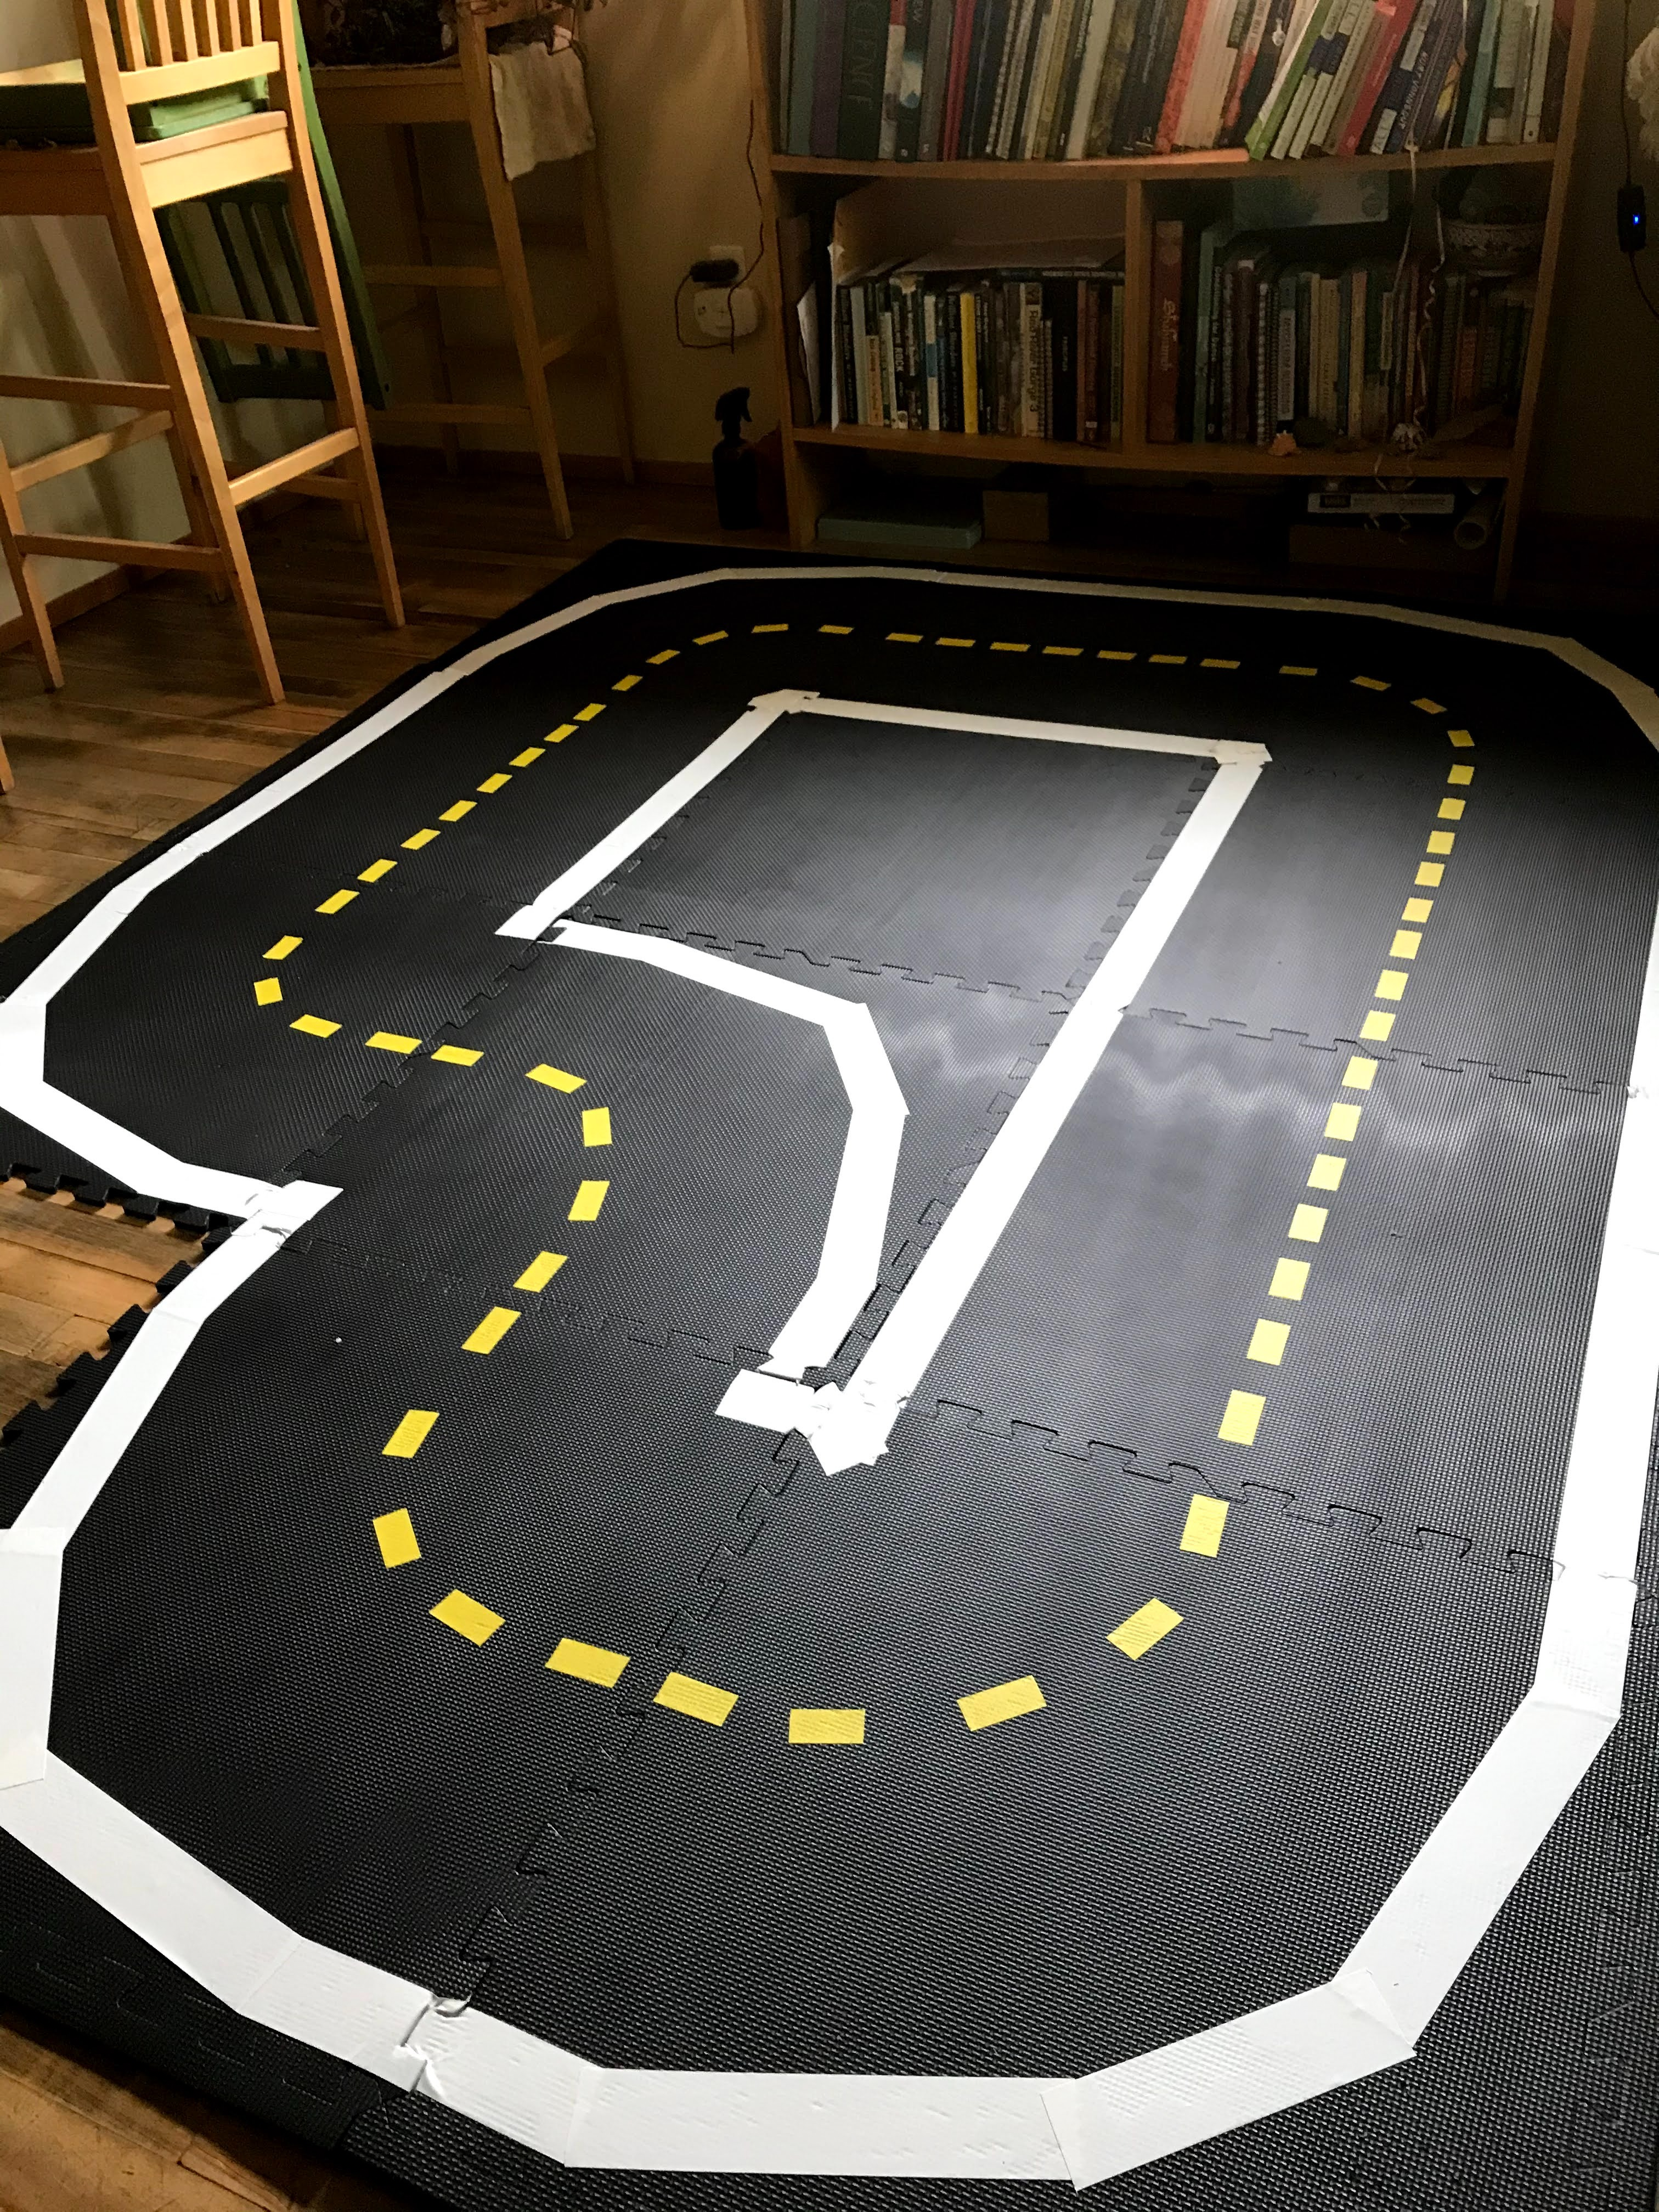
\includegraphics[angle=270,width=8cm,keepaspectratio]{map2_real}
\centering
\caption{Photo of physical layout of map2.}
\label{fig:map2_real}
\end{figure}

\section{Reinforcement Learning Approach}
\todo Discuss our initial approach using RL

\todo how we anticipated this would work

\todo ultimately how it performed poorly

\subsection{DQN}
\todo Discuss general algorithmic idea behind DQN

Unfortunately we were unsuccessful in achieving reasonable training results with this method, with our agent consistently showing an inability to increase average reward obtained despite experimenting with domain randomization in the simulator, training across multiple maps, and performing hyperparameter search (Figure \ref{fig:dqn_training}).

\url{https://youtu.be/SDZ59_2zhGg}

\subsection{DDPG}
\todo Discuss general algorithmic idea behind DDPG

\url{https://youtu.be/1xL8b2MK6N4}

\section{Behavior Cloning Approach}
\todo High level overview of behavior cloning and end-to-end control with monocular images

\subsection{Data Preparation}

\todo Discuss data collection procedure and cleaning
\begin{figure}[H]
\centering
    \subfloat[\centering Simulated data]{{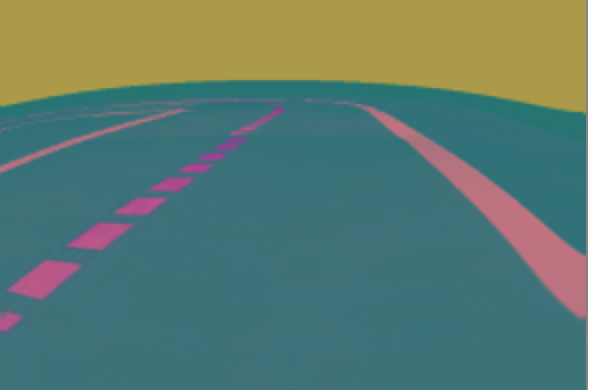
\includegraphics[width=5cm]{sim_data} }}
    \qquad
    \subfloat[\centering Public log data]{{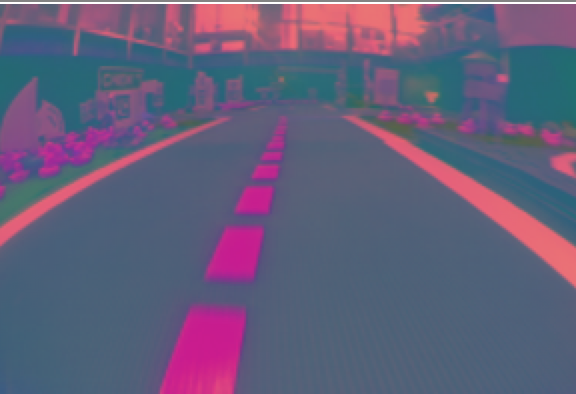
\includegraphics[width=5cm]{log_data} }}
    \qquad
    \subfloat[\centering Custom data]{{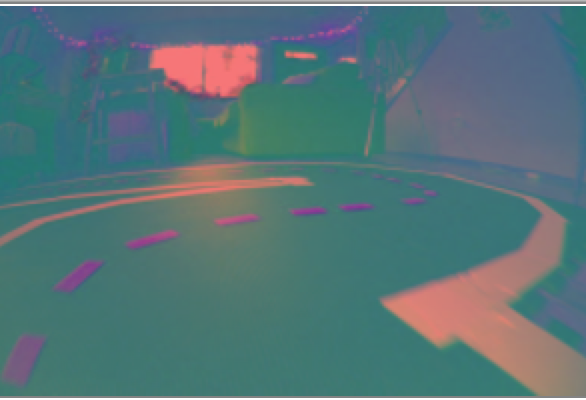
\includegraphics[width=5cm]{custom_data} }}
    \caption{Example frames from the three different data sources used for training. Observations are downsampled 150x200 pixel RGB images.}
    \label{fig:maps}
\end{figure}

Ultimately we used two final datatsets. The largest (henceforth ``dataset A") was used for training the initial model and consisted of 58,414 total observation frames with associated joystick controls, this was a mix of simulated data collected from \texttt{gym-duckietown} using controls given by a built-in pure pursuit controller (50,337 frames) and real robot data from (8,077 frames). The second dataset (henceforth ``dataset B") was compiled from ROS bags collected from one of our own robots being driven on map2 (Figure \ref{fig:maps}b) consisting of 15,560 total frames with controls provided by a human driver (11,661 frames are traveling counter-clockwise).

\subsection{Model Architectures}

Our experiments were focused around two model architectures, the first was an attempt to reproduce results from NVIDIA \cite{DBLP:journals/corr/BojarskiTDFFGJM16} which we named the ``nvidia" model. In that work the authors learn

\begin{figure}
  \centering
  \raisebox{35pt}{\parbox[b]{.1\textwidth}{modelv0}}%
  \subfloat[][]{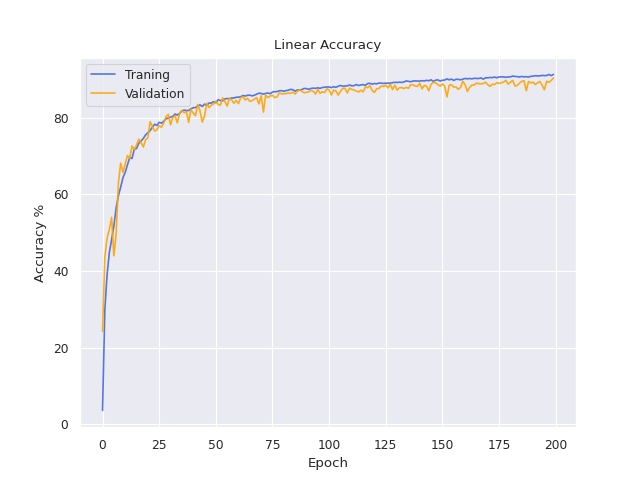
\includegraphics[width=.28\textwidth]{modelv0_linear_accuracy}}\hfill
  \subfloat[][]{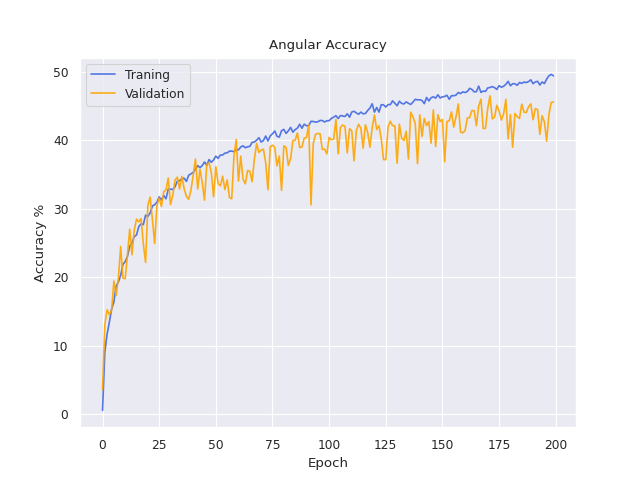
\includegraphics[width=.28\textwidth]{modelv0_angular_accuracy}}\hfill
  \subfloat[][]{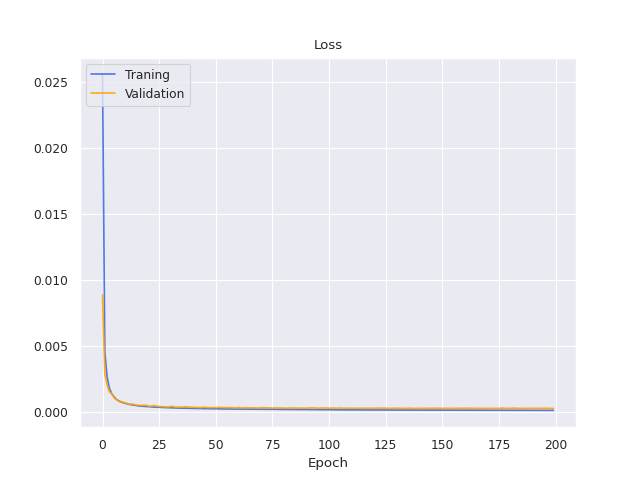
\includegraphics[width=.28\textwidth]{modelv0_loss}}\par
  \raisebox{35pt}{\parbox[b]{.1\textwidth}{modelv1}}%
  \subfloat[][]{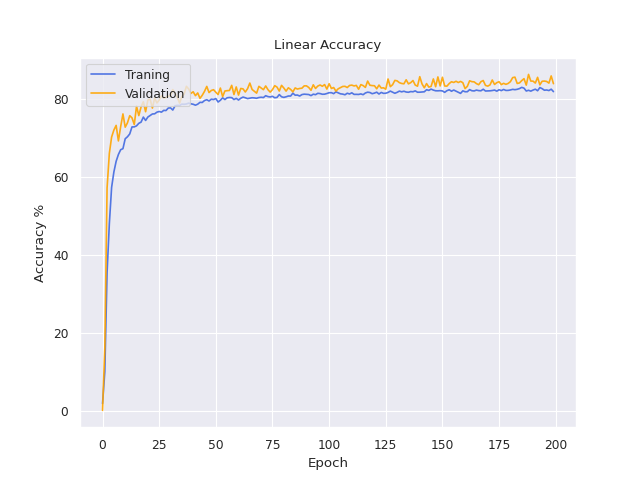
\includegraphics[width=.28\textwidth]{modelv1_linear_accuracy}}\hfill
  \subfloat[][]{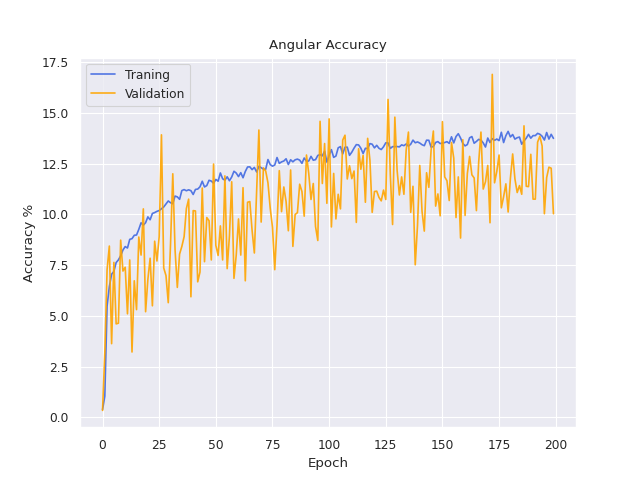
\includegraphics[width=.28\textwidth]{modelv1_angular_accuracy}}\hfill
  \subfloat[][]{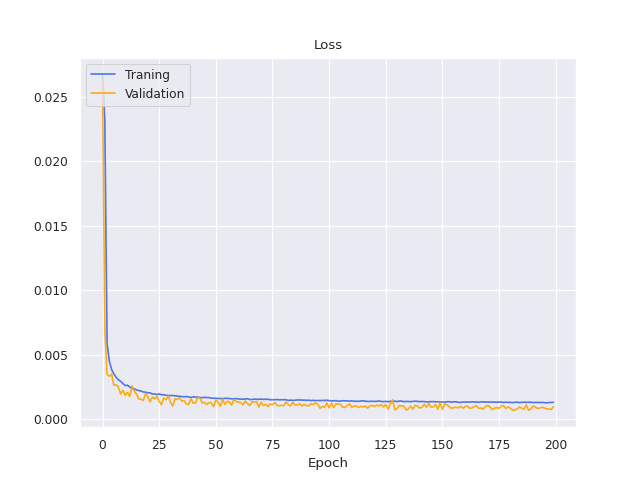
\includegraphics[width=.28\textwidth]{modelv1_loss}}\par
  \raisebox{35pt}{\parbox[b]{.1\textwidth}{nvidia}}%
  \subfloat[][]{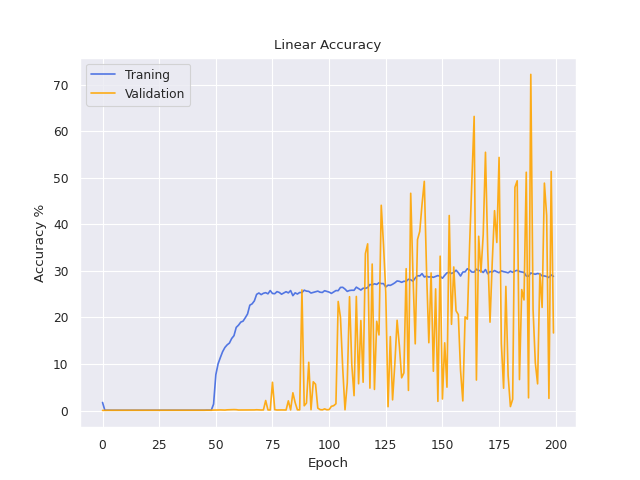
\includegraphics[width=.28\textwidth]{nvidia_linear_accuracy}}\hfill
  \subfloat[][]{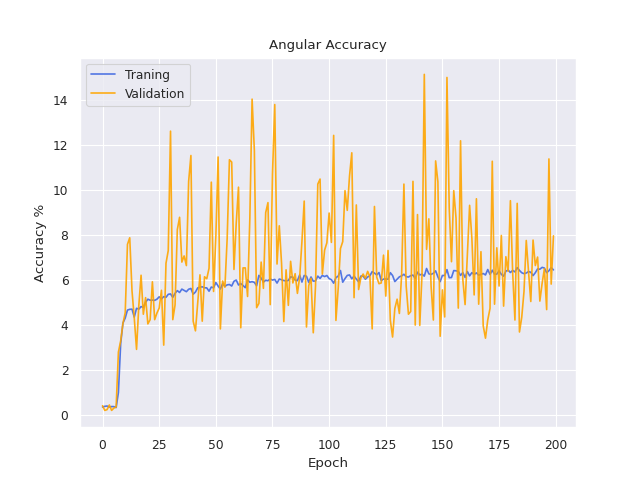
\includegraphics[width=.28\textwidth]{nvidia_angular_accuracy}}\hfill
  \subfloat[][]{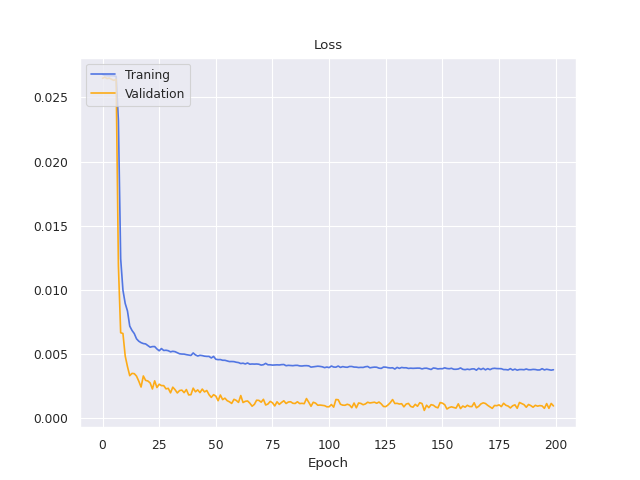
\includegraphics[width=.28\textwidth]{nvidia_loss}}
  \caption{Results from training the three different model architectures on dataset A, showing loss, linear accuracy, and angular accuracy achieved. A prediction was considered correct if the continuous velocity value was within 5\% of the label value.}
  \label{fig:training_results}
\end{figure}

% \begin{figure}[H]
%   \centering
%   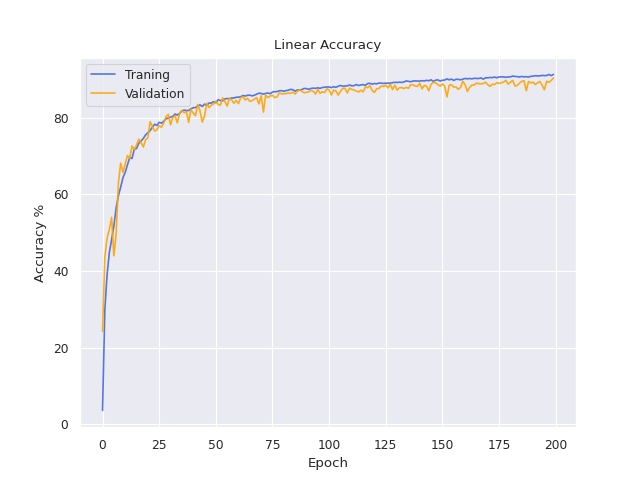
\includegraphics[width=5cm]{modelv0_linear_accuracy}
%   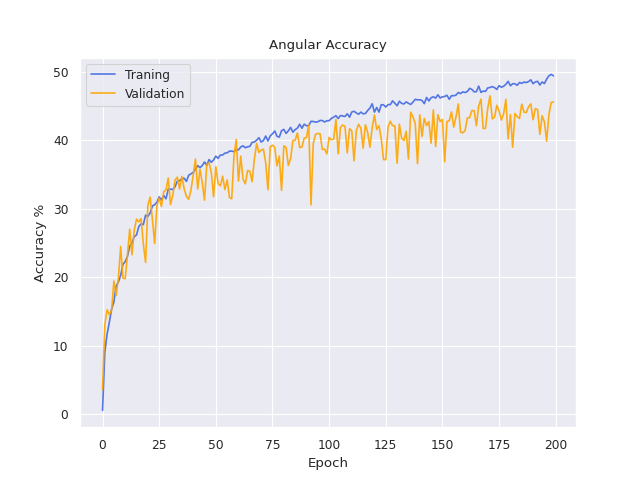
\includegraphics[width=5cm]{modelv0_angular_accuracy}
%   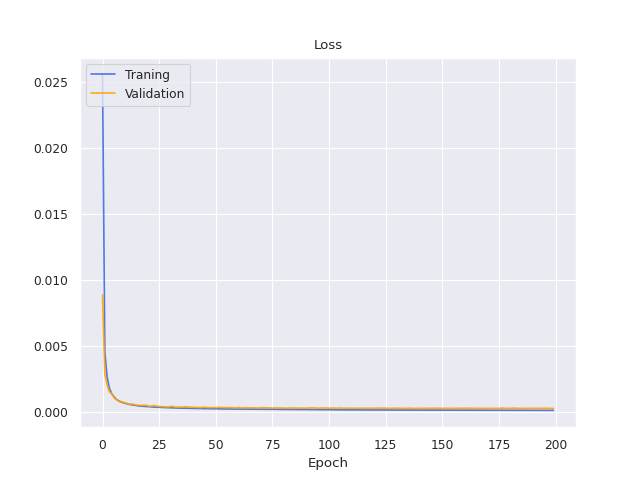
\includegraphics[width=5cm]{modelv0_loss}

%   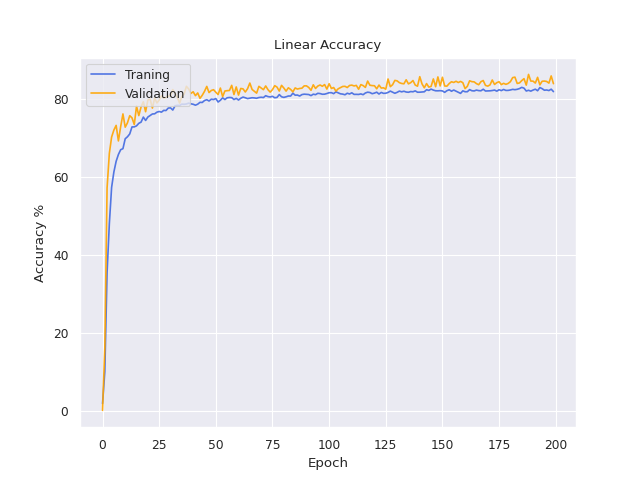
\includegraphics[width=5cm]{modelv1_linear_accuracy}
%   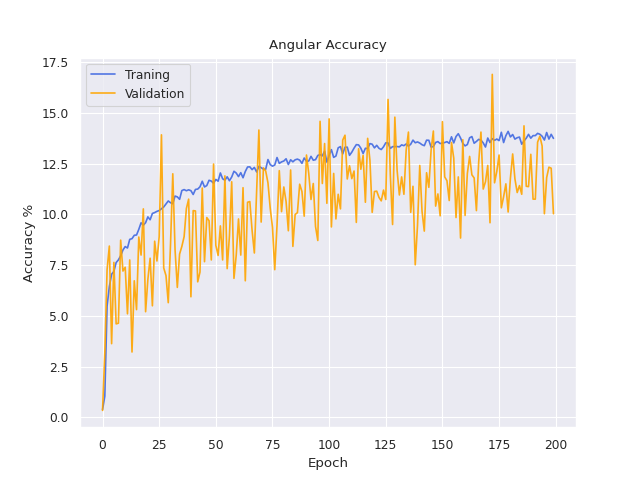
\includegraphics[width=5cm]{modelv1_angular_accuracy}
%   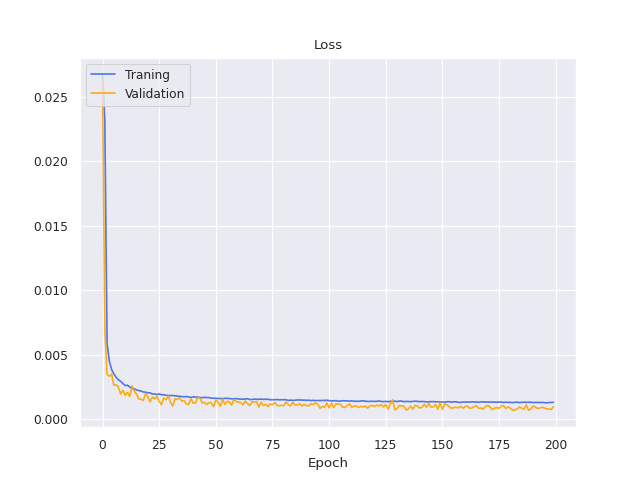
\includegraphics[width=5cm]{modelv1_loss}

%   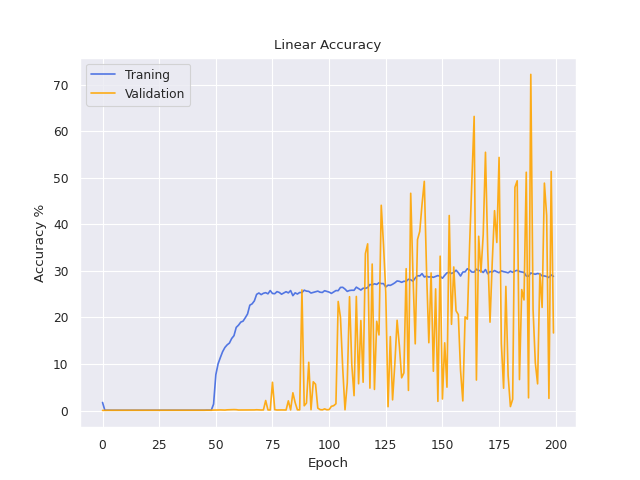
\includegraphics[width=5cm]{nvidia_linear_accuracy}
%   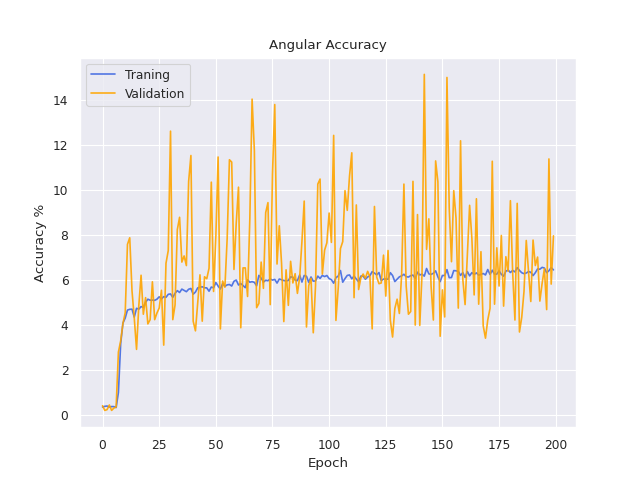
\includegraphics[width=5cm]{nvidia_angular_accuracy}
%   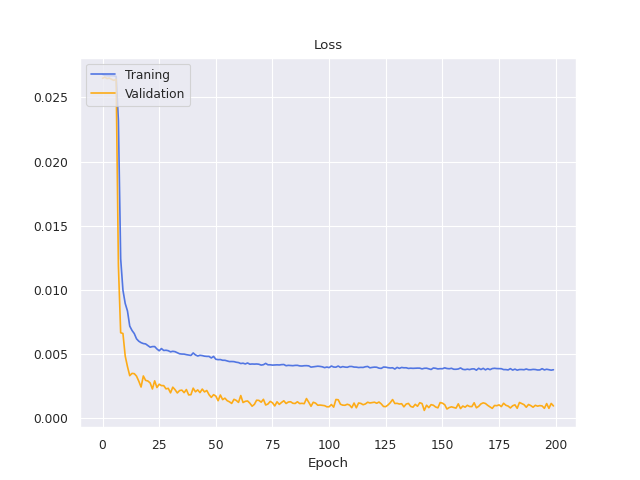
\includegraphics[width=5cm]{nvidia_loss}
% \end{figure}

\todo Discuss each model architecture evaluted

\todo Show data from training

\section{Performance Evaluation}
\subsection{Simulator and AIDO}
\todo Share links to videos from simulator and AIDO submissions

\todo Discuss quantative performance for each model including baseline

\subsection{Real World}

\todo Discuss quantative performance for each model including baseline

\todo Share links to videos for each map/model evaluated

Baselines map2:
\url{https://youtu.be/oNrlfTRxNy0}

Model v1 map2:
\url{https://youtu.be/NMiHz7VIw_4}

\section{Potential Future Improvements}

\todo Discuss algorithmic enhancements

\todo Discuss robot limitations

\bibliographystyle{alpha}
\bibliography{paper}

\end{document}
